
% This template has been edited from the IEEE template available at:
% https://www.ieee.org/conferences/publishing/templates.html
%
% For further help, you may wish to see:#
% https://www.overleaf.com/learn/latex/tables
% https://www.overleaf.com/learn/latex/Inserting_Images
% https://www.overleaf.com/blog/532-creating-and-managing-bibliographies-with-bibtex-on-overleaf

\documentclass[conference]{IEEEtran}
%\IEEEoverridecommandlockouts
% The preceding line is only needed to identify funding in the first footnote. If that is unneeded, please comment it out.
\usepackage[a4paper, total={6in, 8in}, margin=0.75in]{geometry}
\usepackage{cite}
\usepackage{amsmath,amssymb,amsfonts}
%\usepackage{algorithmic}
\usepackage{algorithm} 
\usepackage{algpseudocode} 
\usepackage{graphicx}
\usepackage{textcomp}
\usepackage{xcolor}
\usepackage{wrapfig}
\usepackage{subcaption}
\usepackage{comment}

\def\BibTeX{{\rm B\kern-.05em{\sc i\kern-.025em b}\kern-.08em
    T\kern-.1667em\lower.7ex\hbox{E}\kern-.125em}}

    
\begin{document}

\title{Report Title: Be Descriptive}

\author{
    \IEEEauthorblockN{Student Number}
    \and
    \IEEEauthorblockN{Student Number}
}

\maketitle

\begin{abstract}
It is normal to write the abstract last.  First, try to concisely state the problem/question/challenge under investigation.  Second, state what you found out.  The abstract should help a reader decide if they are interested in reading the whole paper.  
\end{abstract}

% 纤维约束型执行器的原理就是通过纤维约束一个方向或者一部分的弹性体形变,从而使弹性体形变时形成想要的形状。
% 本文的主题就是研究约束纤维方向对弹性体形变的影响
% 

\section{Introduction}

% 用于软机器人执行器的材料通常是各向同性的(intrinsically isotropic),即,面对外力的刺激,其各部分的应变特性是几乎相等的,这一特性使得用单一材料制成的软机器人执行器难以表现出复杂的行为。但是,如果通过引入其他材料进行约束,就可以一定程度上克服这一缺点(1)。比较适合用于进行这一约束的材料主要是各种纤维。纤维材料由于其柔韧性和柔软性(flexibility and softness),以及其作为一种常用材料的事实,使其成为一种非常适于为软机器人引入各向异性的材料。

\begin{wrapfigure}{l}{0.2\textwidth}
  \label{fig:Elastomer}
  \centering
  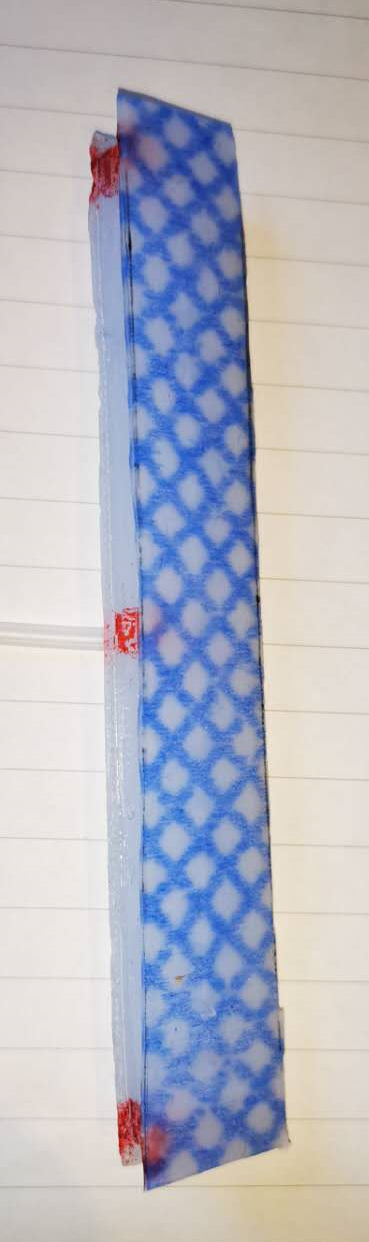
\includegraphics[width=0.15\textwidth]{pics/弹性体示意图.png}
  \caption{Elastomer gripper. The blue grid at the bottom is the strain limited layer.}
\end{wrapfigure}

The materials used for soft robot actuators are typically intrinsically isotropic, meaning that the strain characteristics of their various parts are almost equal in response to external stimuli. This property makes it difficult for a soft robot actuator made of a single material to exhibit complex behavior. However, this drawback can be partially overcome by introducing other materials as constraints. Fiber materials, due to their flexibility and softness, as well as the fact that they are a commonly used material, make them a very suitable material for introducing anisotropic properties into soft robots \cite{overview}.



% 本文中将对布里斯托大学 MSc Robotics 课程 Soft Rbotics 提供的纤维补强执行器进行研究(此处插入图片解释,全貌,受压力的形变效果)。作为一种用压力限制层(nature那个)来补强的纤维补强弹性体,其压力限制层位于长方体弹性体的一个长侧面上。有趣的是,虽然压力限制层是为了给各向同性的弹性体引入约束使其具有一定程度的各向异性特性,但是课程模组本身所提供的压力限制层(Wilco all purpose cloths)也具有各向异性,其受到水平方向拉力时产生的应变可以分解为两个正交的轴向,在一轴上较易发生轴向的应变,在另一轴上则较不容易发生轴向的应变。这就导向了一个问题:压力限制层的方向会对纤维增强弹性体的应变特性产生什么影响?
This article focuses on the fiber-reinforced gripper provided in the Soft Robotics module of the MSc Robotics program at the University of Bristol (Fig. 1). As a fiber-reinforced elastomer with a strain limited layer\cite{stress_constraint_layer}, which is placed on one of the sides of the rectangular elastomer, the interesting point is that although the strain limited layer is introduced to provide some degree of anisotropic properties to the isotropic elastomer, the stress limited layer provided in the course module  (Wilco all purpose cloths) itself is also anisotropic. When subjected to a horizontal tensile force, the cloths' strain can be decomposed into two orthogonal axial components, with axial strain being more easily generated in one axis than in the other. This leads to the question: how does the direction of the strain limited layer affect the strain characteristics of the fiber-reinforced elastomer?


\begin{figure}[htbp]
  \centering
  \begin{subfigure}[b]{0.25\linewidth}
    \centering
    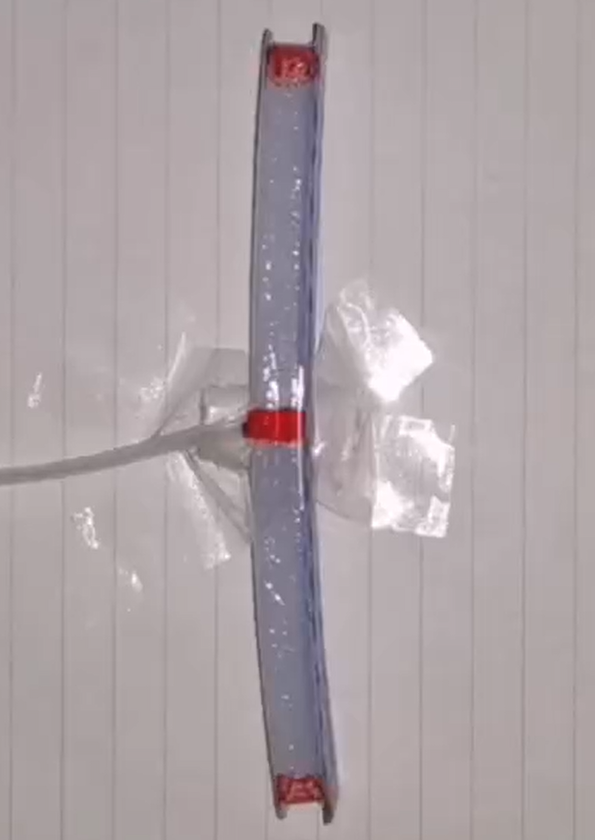
\includegraphics[width=\linewidth]{pics/变形1.png}
    \caption{}
    \label{fig:image1}
  \end{subfigure}
  \begin{subfigure}[b]{0.25\linewidth}
    \centering
    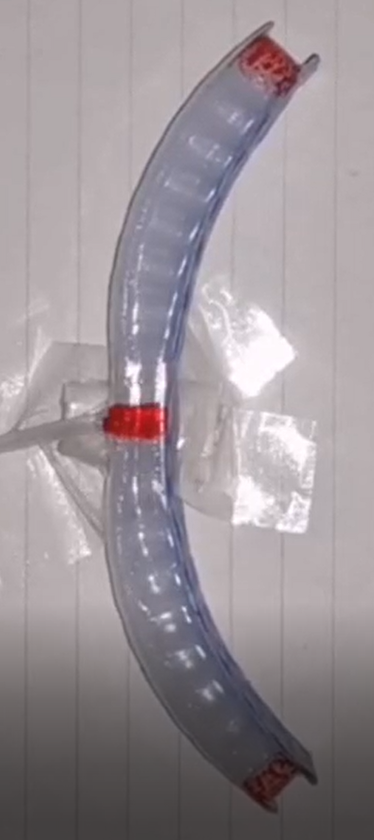
\includegraphics[width=\linewidth]{pics/变形2.png}
    \caption{}
    \label{fig:image2}
  \end{subfigure}
  \begin{subfigure}[b]{0.25\linewidth}
    \centering
    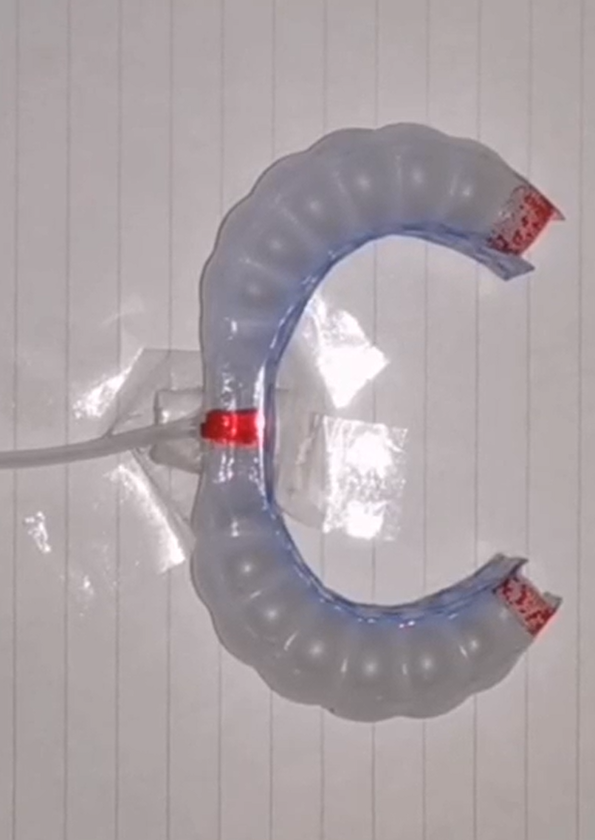
\includegraphics[width=\linewidth]{pics/变形3.png}
    \caption{}
    \label{fig:image3}
  \end{subfigure}
  \caption{The shape of the elastic gripper changes with inflation. The strain limited layer is located on the right side.}
  \label{fig:three_images}
\end{figure}





\subsection{Hypothesis Statement}

% 基于以上描述,本文的假想是:使用各向异性的压力限制层来强化执行器的时候,压力限制层的方向会影响弹性体的应变特性。

Based on the description above , the hypothesis of this study is:
\begin{quote}
When using an anisotropic stress limited layer to reinforce the actuator, the direction of the stress limited layer will affect the strain characteristics of the actuator.
\end{quote}

% 此设想是受(2)启发,由于纤维补强型执行器的原理就是用纤维的应变特性来限制弹性体某一方向的形变,使其不对称从而对其进行某种物理编程(cite那个通过改变纤维角度对其进行物理编程)。对于本文中所使用的具体执行器来说,就是压力限制层会限制弹性体一侧的变形,从而使得弹性体在受到内部气压的时候向一侧弯曲,从而使其产生适合抓握的形状。如果本文的假设成立的话,此执行器就有可能通过在不同位置将压力限制层的方向对其进行进一步的物理编程,如在特定位置放置关节,使其更适合抓握。

This hypothesis is inspired by \cite{mechanical_programing}, as the principle of fiber-reinforced actuators is to use the strain characteristics of the fibers to limit the deformation of the elastomer in a certain direction, making it asymmetric and allowing for some kind of physical programming \cite{fingerlike}. For the specific actuator used in this study, the strain limited layer restricts deformation on one side of the elastomer, causing it to bend towards another side when subjected to internal pressure, resulting in a shape suitable for grasping. If the hypothesis of this study is confirmed, it may be possible to further physically program this actuator by varying the direction of the pressure-limiting layer at different positions, such as placing joints in specific locations to make the actuator more suitable for grasping.

% 本文中将会先研究压力限制层不同朝向对弹性体形变的影响,若有可见的影响,则测试此种影响用于物理编程的可能性。

This report will first investigate the effect of different orientations of the strain limited layer on the deformation of the elastic body. If there is a visible effect, the possibility of using this effect for physical programming will be tested.

% 本文的结构如下:
% 1.介绍:介绍文章的研究背景与假设
% 2.设计与方法论:描述制造的过程以及实验方法论
% 3.结果与分析:描述并分析实验的结果
% 4.讨论:评价试验结果与假设的关系

The structure of this article is as follows:
\begin{enumerate}
    \item \textbf{Introduction}: Introduce the research background and hypothesis of this article.
    \item \textbf{Design and methods}: Describe the actuator manufacturing process and experimental methodology.
    \item \textbf{Results and analysis}: Describe and analyze the results of the experiment.
    \item \textbf{Discussion}: Evaluate the relationship between the experimental results and the hypothesis.
\end{enumerate}


\section{Design and methods}

\begin{comment}

\begin{algorithm}
	\caption{PPO}\label{pseudo:ppo}
	\begin{algorithmic}[1]
		\For {$iteration=1,2,\ldots$}
			\For {$actor=1,2,\ldots,N$}
				\State Run policy $\pi_{\theta_{old}}$ in environment for $T$ time steps
				\State Compute advantage estimates $\hat{A}_{1},\ldots,\hat{A}_{T}$
			\EndFor
			\State Optimize surrogate $L$ wrt. $\theta$, with $K$ epochs and minibatch size $M\leq NT$
			\State $\theta_{old}\leftarrow\theta$
		\EndFor
	\end{algorithmic} 
\end{algorithm}

It can be a good idea to include pseudocode (see Algorithm \ref{pseudo:ppo} above), and you may also want to include equations such as eq.\ref{eq:emc2} below:

\begin{equation}\label{eq:emc2}
E=mc^2
\end{equation}

\end{comment}

% 为了对比应变限制层方向对弹性体形变的影响,本文将采用如下所述的方法。
To compare the effect of the orientation of the strain limited layer on the deformation of the elastomer gripper, the following method will be used in this study.

\subsection{Overview of Method}

\begin{comment}
    
Describe to the reader the general structure and procedure of your experiment. You should provide a specification a bit like a cake recipe.  For example: how long does your experiment last?  how many repeated trials do you use?  how many alternate scenarios are there?
\end{comment}

% 首先定义应变限制层的方向:相同大小的拉伸外力从不同方向作用于应变限制层时,能使应变限制层应变最大化的施力方向就是应变限制层的方向。
Firstly, the direction of the strain limited layer is defined as follows: when the same magnitude of tensile force is applied to the strain limited layer from different directions, the direction that maximizes the strain of the strain limited layer is defined as the direction of the strain limited layer.

% 为了减少实验中大量无关变量的干扰,采用的方法是:在同一抓握器的两个手指上使用不同方向的应变限制层。其中一根手指采用正常的方向(从指根指向指尖),另一根手指的应变限制层则相对正常方向有一定的倾斜。倾斜的具体角度分别为45°和90°。
To reduce the interference of a large number of irrelevant variables in the experiment, the method employed was to use strain limited layers of different directions on two fingers of the same gripper. One finger is using the normal direction (pointing from the root to the tip of the finger), while the strain limited layer on the other finger is tilted at a certain angle relative to the normal direction. The specific angles of inclination were 45° and 90°, respectively.


% 插入图片

\subsection{Discussion of Variables}
You should outline the key variables within your experiment. This will help your reader to later believe your results are credible and not confused.
\begin{itemize}
    \item \textbf{Controlled Variables}: These are the parts of your experiment (task, hardware, software, environment) which \emph{could} vary, but which you have controlled by careful design of your experiment.  For example, battery life varies, so you will use new batteries.
    \item \textbf{Independent Variable}: This is the part of your experiment which you are changing so that you hope to observe a measurable alteration in performance.  Note that, we ever only want one independent variable - sometimes we aim for this, but concede other parts will change, and we need to make careful analysis of our system and/or results.
    \item \textbf{Dependent Variable(s)}: These are the part(s) of your experiment in which you hope to observe a measurable change.  You will design or select appropriate \emph{metrics} to measure and analyse this dependable variable.  For example, we can have one dependent variable of the system, but use metrics of mean, mode and median to analyse it.
\end{itemize}

\subsection{Discussion of Metric(s)}

 In this section you should discuss the rationale (why) you have selected your metric(s) - e.g. how do these metrics help us to interpret your results?  Your metric(s) will need to be applied consistently throughout your experiment for them to provide a comparison of performance.  
 
 You should discuss the advantages and disadvantages of your metric(s).  Often, we need more than one metric to compensate for the information which is confused or hidden in another metric.  By using more than one metric, we can get closer to the truth of the outcome of your experiment.  

\section{Results}

In this section you should present your results.  In general, it is best to aim for both \emph{quantitative} results (e.g., data) and \emph{qualitative} results (e.g., a written observation or graphic which is representative).  

You should use subsections where they aid in clarity.  For instance, it may be useful to present results for a ``baseline" system, then a results for an ``improved" system, and then finally results which consider both ``baseline" and ``improved" systems together.  However, this will depend entirely on your project and how you have designed your experiment.

When presenting results, aim for a presentation which clearly communicates an insight. For example, a large table of all the individual data requires the reader to do a lot of work to find out what is important.  In contrast, a table which appropriately presents the mean and standard deviation has summarised the results for the reader (and would be more useful).  Similarly, aim to combine data onto a chart when possible so that a direct comparison can be made - and when possible, include error bars.  

\begin{figure}[htbp]
\centerline{\includegraphics{fig1.png}}
\caption{Example of a figure caption.  This dot may or may not be circular.}
\label{fig1}
\end{figure}

Remember to label all axis, caption all graphs, figures and tables, and to reference these elements in the report text (e.g. see figure \ref{fig1}) - never require a reader to have to come to their own conclusion or understanding, explain what they are looking at.  Remember to attempt to give an explanation for any anomalies in your results.  


\section{Discussion and Conclusion}

Begin your discussion and conclusion by re-stating your hypothesis.  You can literally copy-and-paste your hypothesis here.  

Because the VL1680X has been identified as an active sensor with ... limitations, we hypothesised that:
\begin{quote}
    by applying ... filtering to the sensor, we predict a measurable improvement of the sensor under ... conditions.  
\end{quote}

Make a discussion of what your results showed - whether this supported or refuted your hypothesis.  It may be that the results were mixed (supporting and refuting) and you should discuss that here. In your discussion, use this as another opportunity to demonstrate/evidence your understanding. Try to avoid stating the obvious - instead, use analysis/evaluation/synthesis to show that you understand \emph{how} and \emph{why} you saw the results you did.  What are the implications of your findings?  

This is also a good opportunity to evaluate your experiment and project as a whole.  You may wish to further discuss the limitations of the study (e.g. the difficulty of controlled/dependent variables, or any problems you faced in your project).  You may wish to make a recommendation for future work - but ensure that this is a clear advancement from the understanding you have gained and not wild speculation.


\bibliographystyle{ieeetr} 
\bibliography{ref}


\end{document}
